%Background body
%Created MS 05-11

\section{Background}\label{background}

\subsection{Optical Pumping}

Optical pumping is the process in which the interaction of light with
atoms produces a population of energy levels that is distinct from the
thermal equilibrium Boltzmann distribution \cite{bernheim}. In a
three-state system, with a ground state $|g\rangle$, excited state
$|e\rangle$, and intermediate metastable state $|m\rangle$
(Fig. \ref{pumping}), it is possible to selective populate the metastable
state if the natural decay time $\gamma_{rel}$ is sufficiently long in
comparison to the pumping time. If laser light is applied on resonance
with the $|e\rangle$ to $|g\rangle$ transition, it drives the atom
population to the excited state, and then the atoms decay to the lower
energy levels with some time constant. If the laser light cannot
excite atoms from the metastable state to the excited state (for
example, due to selection rules), the process preferentially populates
the state $|m\rangle$, resulting in optical pumping.


\begin{figure}[h]
\begin{center}
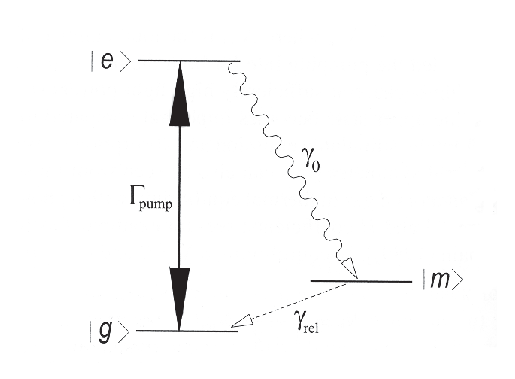
\includegraphics[width=4in]{figures/pumping.eps}
\caption{\small{Three level system with optical pumping rate $\Gamma_{pump}$}}
\label{fig:pumping}
\end{center}
\end{figure}


\subsection{Rubidium System}

In this experiment, we consider an ensemble of rubidium atoms as an
optical pumping system. Rubidium is an alkali atom with a single
electron in its outer shell, and thus can be modelled as a
hydrogen-like system. Here, we take the outer $5^2S_{1/2}$ level as
the ground state and focus on the $D_1$ transition between the
$5^2S_{1/2}$ and $5^2P_{1/2}$ states. 

We use a natural abundance Rubidium cell for optical pumping, which
consists of $72\%$ $^{85}$Rb and $28\%$ $^{87}$Rb, so we are able to
investigate the properties of both isotopes. The energy level diagrams
are presented in Fig.~\ref{fig:8587levels}.


\begin{figure}[h]
\begin{center}
\subfigure[$^{87}$Rb energy spectrum]{\label{fig:edge-b}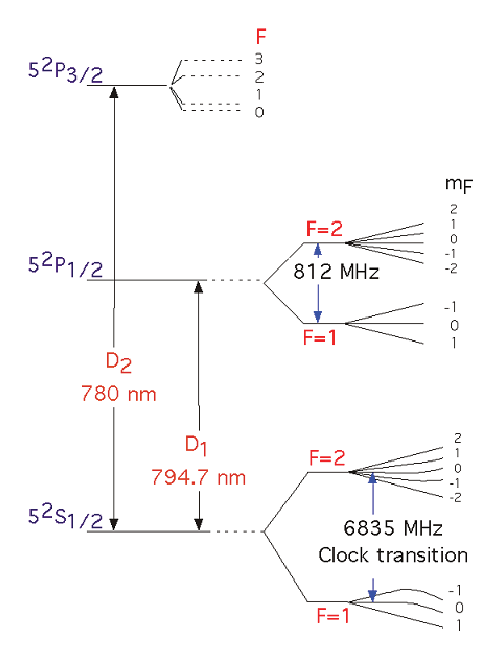
\includegraphics[height=3.5in]{figures/87levels.eps}}
\hspace{-1mm}
\vspace{-2mm}
\subfigure[$^{85}$Rb energy spectrum]{\label{fig:edge-a}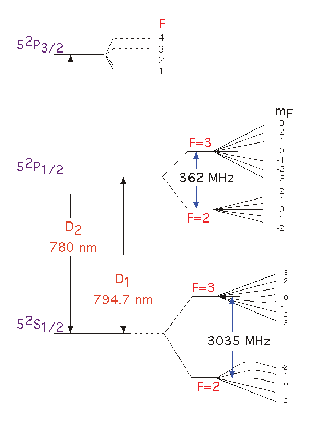
\includegraphics[height=3.5in]{figures/85levels.eps}}
\vspace{-2mm}
\caption{\small{CAPTION GOES HERE}}
\label{fig:8587levels}
\end{center}
\end{figure}

There are several levels of splitting which occur in the Rb atom. The
splitting of the $5^2P$ state into $5^2P_{1/2}$ and $5^2P_{3/2}$ is
due to spin-orbit coupling, that is, the addition of the spin and
orbital angular momenta ($S$ and $L$, respectively) of the electrion
to comprise the total angular momentum $J$. As mentioned above, the
laser has been tuned to the $D_1$ line because of its better optical
pumping properties (Fig.~\ref{fig:8587levels}).

In addition, each total electron angular momentum level is further
split by the coupling of spins of the electron to the nucleus, known
as hyperfine splitting. This results in the distinct $F$ levels, where
$F = I + J$; $I$ is the spin of the nucleus and $J$ as above is the
total electron angluar momentum. Each pair of $F$ states in these
levels of Rb is separated by a frequency shift on the order of
hundreds or thousands of MHz, allowing the tuning of the laser to a
particular transition (Fig.~\ref{fig:fluor}). For instance, we
chose to focus on the $^{85}$Rb $5^2S_{1/2}, F = 3$ to $5^2P_{1/2}, F
= 3$ transition for most of the experiment, because the density of the
$^{85}$Rb isotope is over twice as high, and the $3$ to $3$ line is
more easily separated from the neighboring transitions.

\begin{figure}[h]
\begin{center}
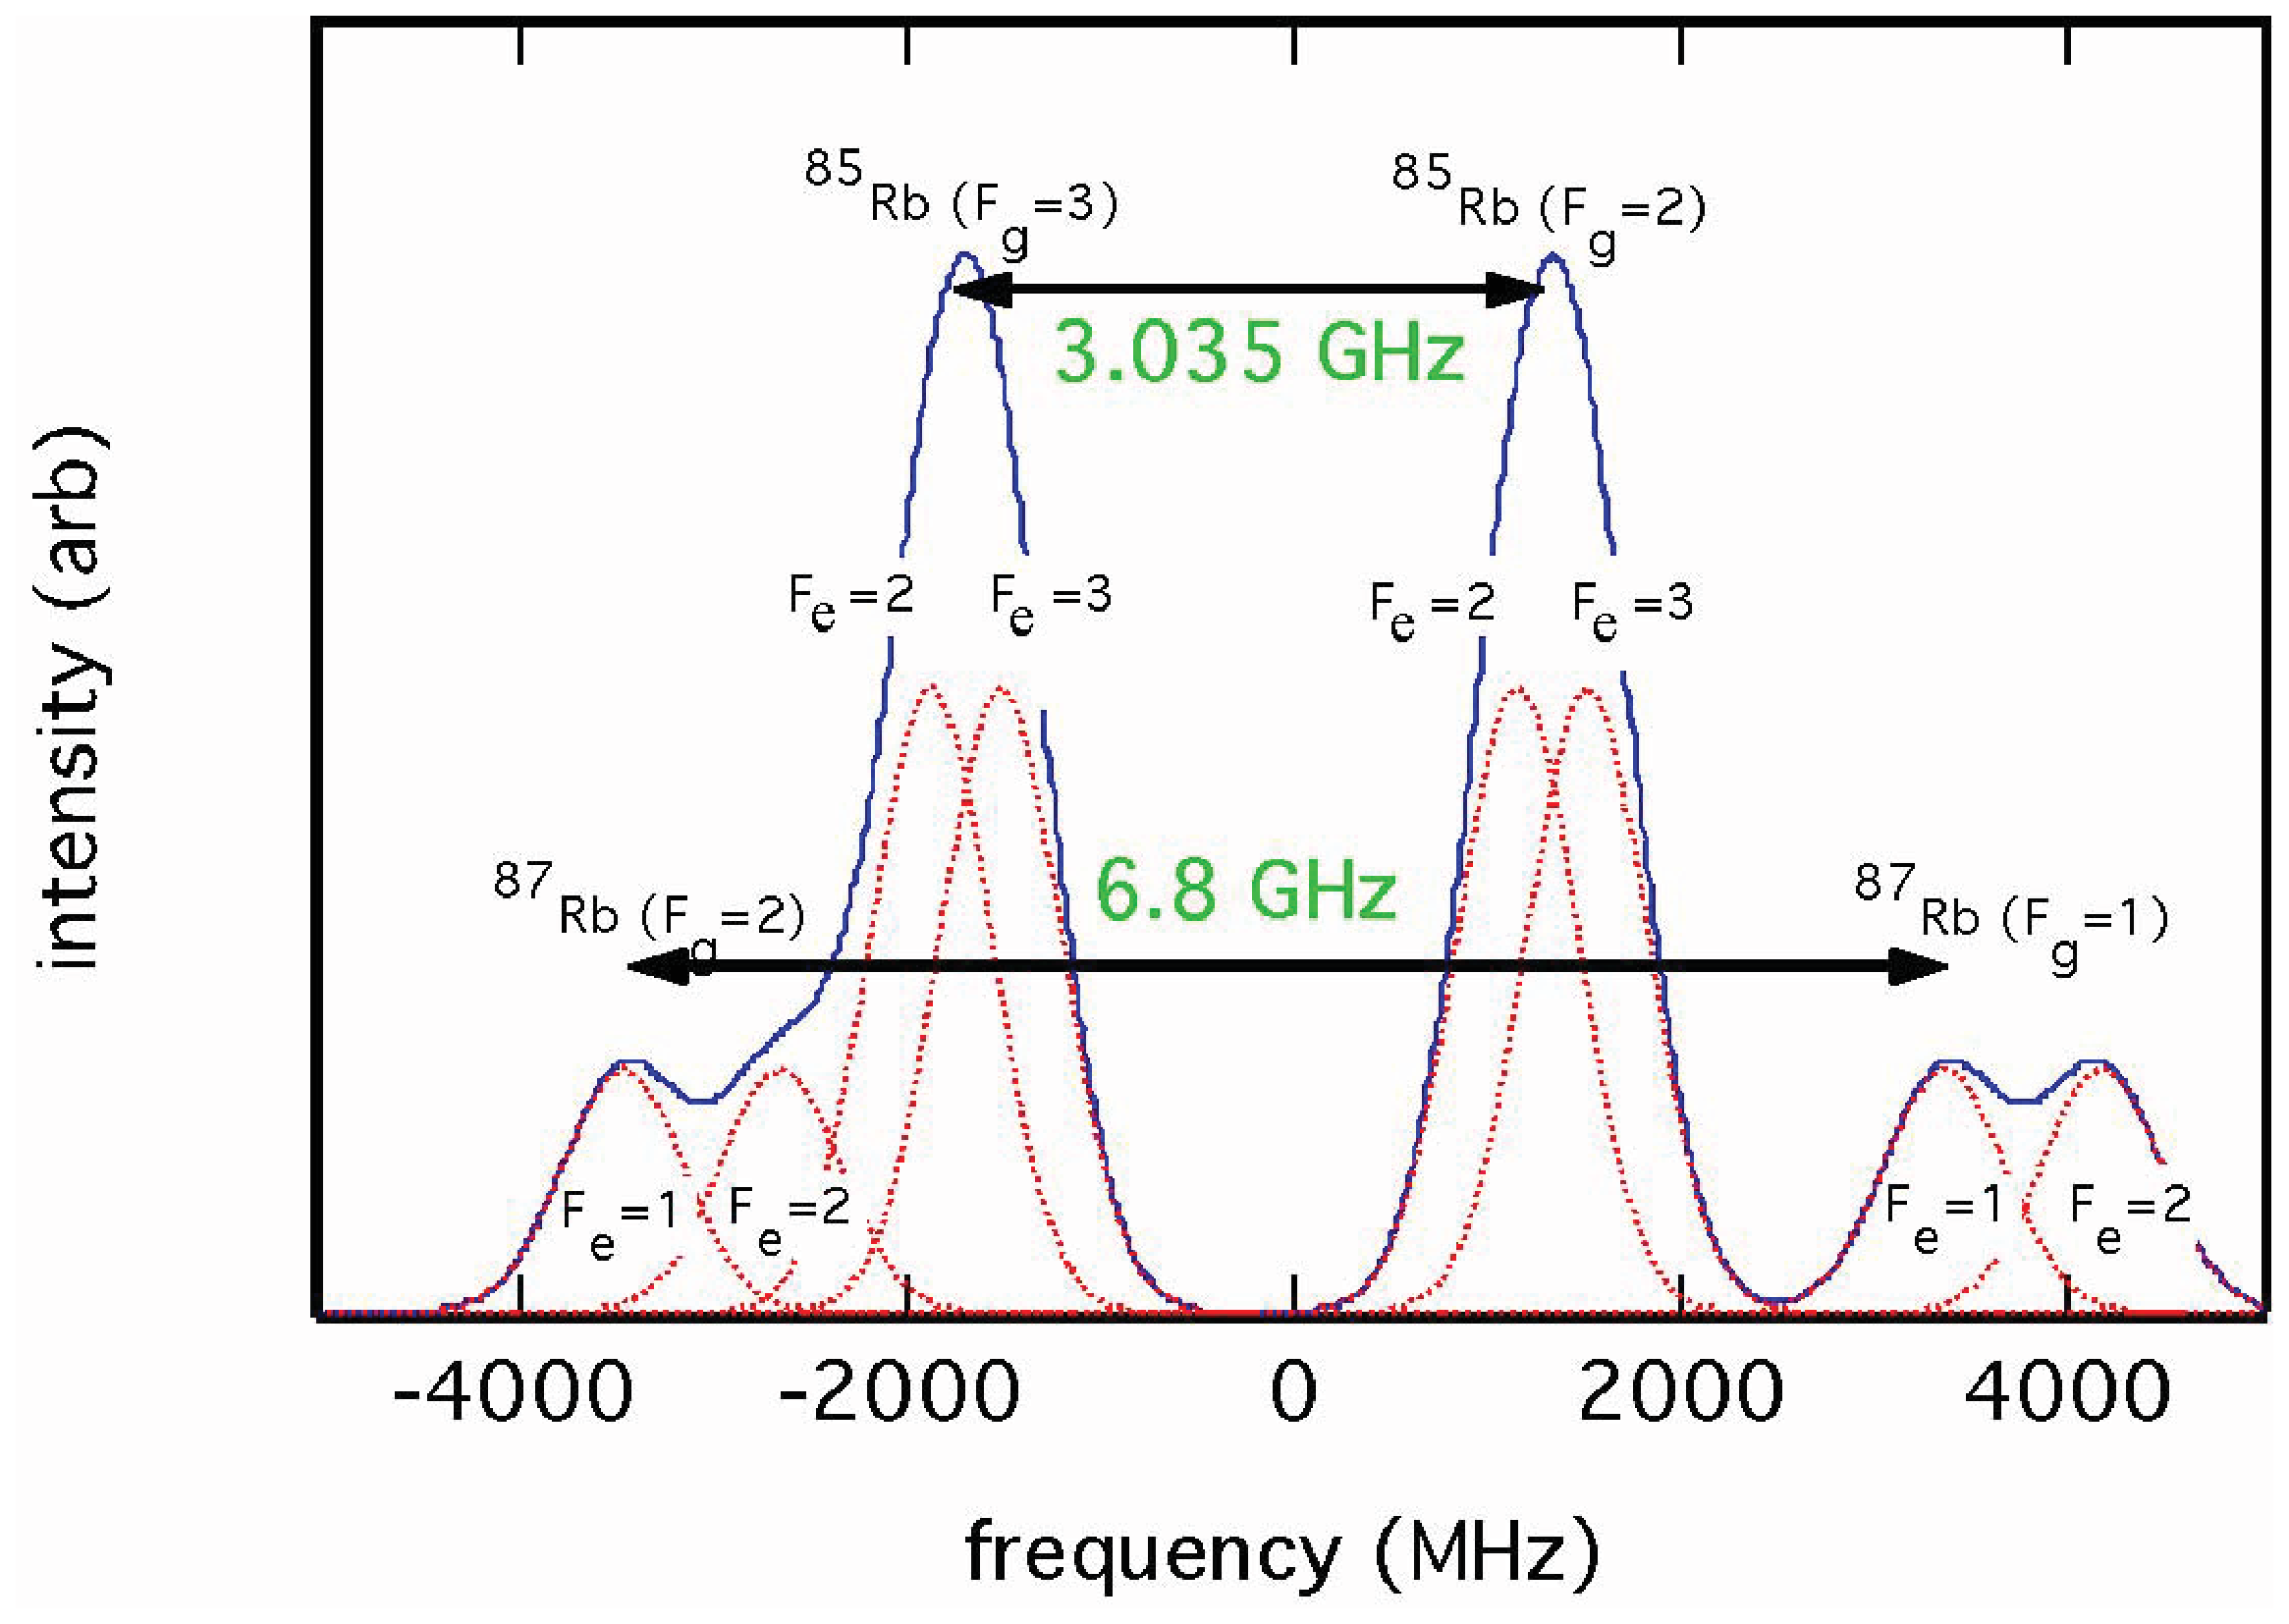
\includegraphics[height=3in]{figures/fluorescence.eps}
\caption{\small{Fluoresence spectrum of natural abundance rubidium. The $x$-axis is a relative measure of frequecy, with $0$ being the $D_1$ transition frequency. The dashed red line represents the fluorescence from individual transitions, and the blue line is the combined intensity.}}
\label{fig:fluor}
\end{center}
\end{figure}

Further splitting occurs in the Zeeman effect, where the degenerate
magnetic sublevels are split via an application of a uniform magnetic
field. For weak fields, the splitting is directly proportional to $B$,
the magnetic field amplitude and the magnetic dipole moment. The
change in the energy is given by

\begin{equation}
\Delta E = g_F\mu_B B m_F
\label{eqn:zeeman}
\end{equation}

where $\mu_B = \frac{e\hbar}{2m_e}$ is the Bohr magneton, $B$ is the
$z$-projection of the magnetic field, and $m_F$ is the spin projection
in the $z$ direction of the total angluar momentum of the atom
\cite{budker }. The qualitative dependence of these splittings on
magnetic field amplitude can be seen in Fig.~\ref{fig:8587levels},
where the energy split between initally degenerate levels increases
with magnetic field.

The general system of optical pumping that we observe works as
follows: circularly polarized light interacts with the rubidium atoms,
and some of them absorb the photons and enter the excited state with
$l_{e}=l_{g}+1$ (the sign depending on the polarization direction of
the light, but chosen here to be positive for simplicity). The excited
atom will spontaneously decay down to any allowed ground state,
\emph{i.e.} $l_{g} = l_{e} \pm 1$. However, the atoms in the most
extreme $+l$ state will not be able to be transferred to the excited
state, as there is no way for them to increase their $l$. As atoms
decay from the excited state into allowed ground states equally, the
ones that fall into $l=l-1$ will be moved back to the excited state
until they decay again. Each time this decay occurs, half the atoms
move into the extreme state, and so eventually all the atoms will be
in this state. Experimentally, this is observable as an increase in
the transmission of the laser through the atoms, as the light is not
absorbed when the atoms are in the extreme, ``dark'' state.


\subsection{Magnetic Interactions}

In order to study the properties of the rubidium atoms, such as the
g-factor, we introduce a magnetic field transverse to the $z$
direction established by the laser and uniform magnetic field. This
field is introduced at a RF on the order of the Zeeman splittings,
coupling the dark state with the ground states. 

\subsubsection{Rabi Oscillations}

For a two-level system with ground state energy $E_2$ and excited
state energy $E_1$, the application of a periodic perturbation of the
form $V(t) = V_0e^{i\omega t}$ with a relaxation (damping) term
proportional to a constant $\Gamma$, the time dependence of the
population of the upper state is given by

\begin{equation}
P(t) = \frac{(2V_0)^2e^{-\Gamma t/2}}{(2V_0)^2 +\Delta^2 + \Gamma^2/4}\sin^2(\frac{t}{2}sqrt{(\Delta + \Gamma/2)^2 + (2V_0)^2}
\end{equation}

Here, $\Delta = \omega - \omega_0$ is the detuning, with $\omega_0 =
(E_1 - E_2)/hbar$ the separation between the upper and lower state of
the system, and $\omega$ the frequency of the periodic
perturbation. $\Gamma$ is the natural decay rate of the population in
the excited state.

This gives the general behavior of a driven, damped optical system. In
the case of a three level system, it is useful to make the
approximation of a small RF perturbation on top of the pumping
system. in that case the logic of the above discussion applies


\subsection{Rate Equations}

\subsubsection{Power Broadening}

\subsubsection{Time Constants}

$\tau$ is the optical pumping time, which is the time it takes to
change the total magnetization from thermal equilibrium to the maximal
equilibrium value with the presence of an external electromagnetic
field.

$T_1 = 1/\gamma_1$ is time constant of longitudinal relaxation,
i.e. the time that the diagonal elements of the density matrix
$\rho_{jj}$ return to the equilibrium in the absence of other
perturbations \cite{vanier} p79.

\begin{equation}
\gamma_1 = \gamma_1^{se} + \gamma_1^{w} + \gamma_1^{bg} 
\label{eqn:gamma1}
\end{equation}

where $\gamma_1^{se}$ is the spin exchange rate, $\gamma_1^{w}$ is the
wall collision rate due to leaving the beam, and $\gamma_1^{bg}$ is
the rate due to buffer gas collisions \cite{vanier}.

$\gamma_2$ is the coherence relaxation rate; the off-diagonal elements
$\rho_{ij}$:

\begin{equation}
\gamma_2 = \gamma_2^{se} + \gamma_2^{w} + \gamma_2^{bg}
\label{eqn:gamma2}
\end{equation}

\subsection{Spin Exchange}


Spin exchange is the ability of two particles to transfer their spin
orientation to one another upon making a collision (needs to be
paraphrased)\cite {bernheim}. The mechanism of spin exchange is one of
the largest factors contributing to the natural linewidth of the RF
resonance. In addition, spin exchange is a valuable technique of
studying the properties of an atom or particle for which a direct
optical particle procedure is much more difficult.

The time between spin exchange collisions is given by

\begin{equation}
T_{se} = 1/\gamma_{se} = (n\overline{v}\sigma_{se})^{-1}
\end{equation}

where $n$ is the vapor density and $\overline{v}$ is the average velocity, given by

\begin{equation}
\overline{v} = \sqrt{\frac{8RT}{\pi m}}
\end{equation}

where $R$ is the ideal gas constant, $T$ is the temperature, and $m$
is the molar mass of the atoms \cite{vanier}. According to Vanier
Table 7.1.1, at $T = 320$ K, $n = 9.935\times 10^{10}$ cm$^{-3}$ and
at $T = 325$ K, $n = 1.545\times 10^{11}$ cm$^{-3}$. At our operating
temperature of $322.75$ K, we can extrapolate the number density to be
approximately  $n = 1.297\times 10^{11}$ cm$^{-3}$. 

In this experiment, we use the spin exchange mechanisms between
$^{85}$Rb and $^{87}$Rb in order to study the contribution of spin
exchange collisions to the inherent RF linewidth of the two isotopes
(Eqn.~\ref{eqn:gamma2}), as well as study the spin exchange cross
section $\sigma_{se}$.

\subsection{Inhomogeneous Broadening}


\begin{figure}[h]
\begin{center}
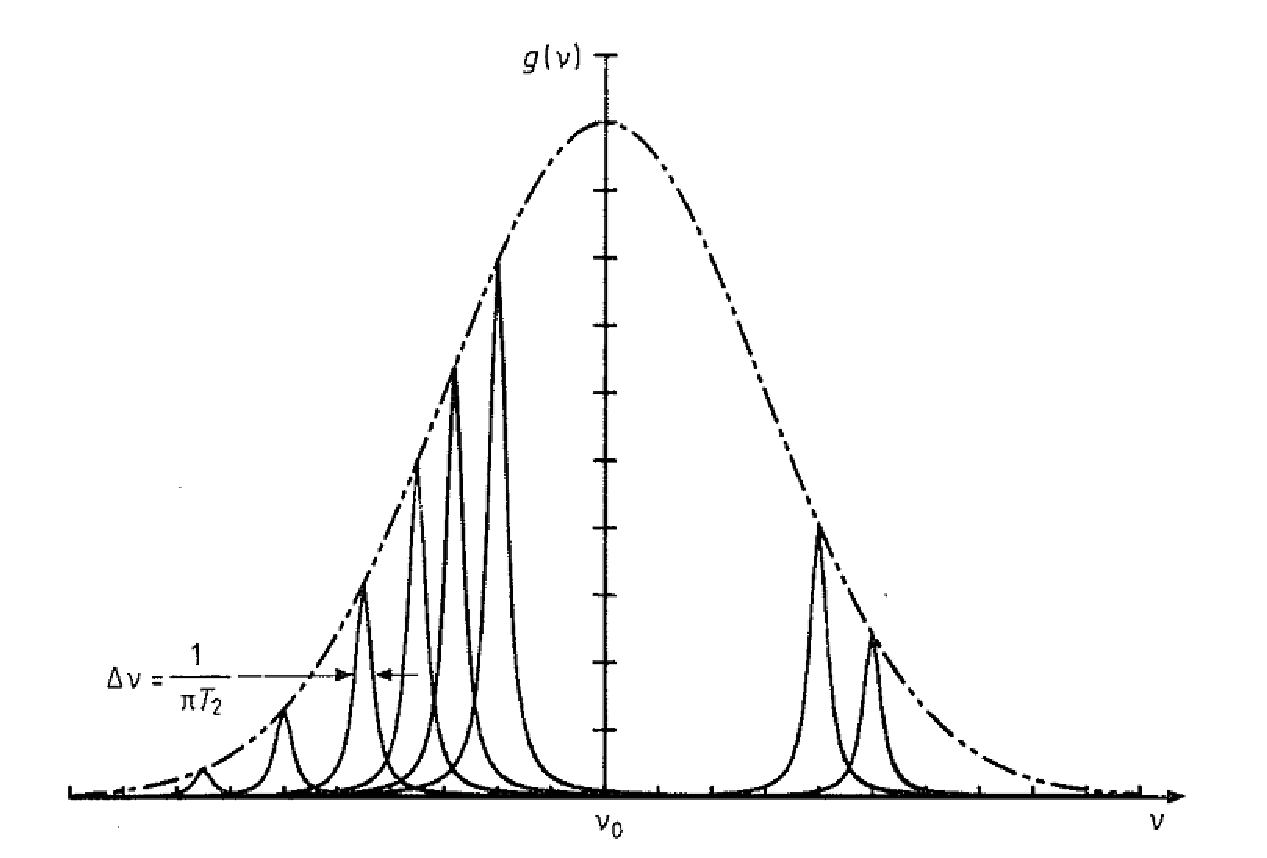
\includegraphics[height=3in]{figures/inhomogeneous.tif}
\caption{\small{In the event of inhomogeneities in the system ($e.g.$ in the uniform magnetic field), the overall linewidth of the RF resonance becomes broadened. The general form of the broadening is shown above, where each portion of the population of atoms is experiences a different B field amplitude and has a different center frequency.}}
\label{fig:inhomo}
\end{center}
\end{figure}


